%%%%%%%%%%%%%%%%%%%%%%%%%%%%%%%%%%%%%%%%%
% Beamer Presentation
% LaTeX Template
% Version 1.0 (10/11/12)
%
% This template has been downloaded from:
% http://www.LaTeXTemplates.com
%
% License:
% CC BY-NC-SA 3.0 (http://creativecommons.org/licenses/by-nc-sa/3.0/)
%
%%%%%%%%%%%%%%%%%%%%%%%%%%%%%%%%%%%%%%%%%

%----------------------------------------------------------------------------------------
%	PACKAGES AND THEMES
%----------------------------------------------------------------------------------------

\newcommand{\CC}{C\nolinebreak\hspace{-.05em}\raisebox{.4ex}{\tiny\bf +}\nolinebreak\hspace{-.10em}\raisebox{.4ex}{\tiny\bf +}}


\newcommand{\Hammer}{\texttt{Hammer\,}}

\documentclass{beamer}
\usepackage[utf8]{inputenc} 
\usepackage[T1]{fontenc}
\usepackage{setspace}
\usepackage{color}
\usepackage{listings}
\usepackage{graphicx} % Allows including images
\usepackage{booktabs} 
\usepackage{xcolor}     % for colour
\usepackage{lipsum}     % for sample text
\usepackage{mdframed}   % for framing



\usepackage{hyperref}
\hypersetup{colorlinks,
citecolor=blue,
linkcolor=.,
menucolor=white,
filecolor=pink,
anchorcolor=yellow
}

\newmdtheoremenv[%
linecolor=gray,leftmargin=60,%
rightmargin=40,
backgroundcolor=gray!40,%
innertopmargin=0pt,%
ntheorem]{myprop}{Proposition}[section]


\mode<presentation> {

\usetheme{AnnArbor}

\usecolortheme{whale}
%\usecolortheme{wolverine}

}


%----------------------------------------------------------------------------------------
%	TITLE PAGE
%----------------------------------------------------------------------------------------

\title[Contributing to Hammer]{Contributing to Hammer: An Introduction} % The short title appears at the bottom of every slide, the full title is only on the title page

\author{Kyle Beyer} % Your name
\institute[UM] % Your institution as it will appear on the bottom of every slide, may be shorthand to save space
{
University of Michigan \\ % Your institution for the title page
\medskip
\textit{\href{mailto:beykyle@umich.edu}{beykyle@umich.edu}} % Your email address
}
\date{\today} % Date, can be changed to a custom date

\begin{document}

\begin{frame}
\titlepage % Print the title page as the first slide
\end{frame}

\begin{frame}
\frametitle{Overview} % Table of contents slide, comment this block out to remove it
\tableofcontents 
\end{frame}

%----------------------------------------------------------------------------------------
%	Section 1: toolchain
%----------------------------------------------------------------------------------------

\section{Introduction}

\begin{frame}
  \frametitle{Introduction to \Hammer}

  \Hammer is a research framework for radiation transport solvers. It is:

  \begin{itemize}
    \item student driven
    \item written in object-oriented \CC17
    \item application agnostic 
    \item lightweight
    \item parallel
  \end{itemize}
\end{frame}

\section{Toolchain}

\begin{frame}
\frametitle{Package Manager}
  
   Use a package manager, unless you like your life to be hard
  \begin{itemize}
    \item Debian/Ubuntu: use \href{https://help.ubuntu.com/lts/serverguide/apt.html}{\texttt{apt}}
    \item MacOS: install \href{https://brew.sh/}{\texttt{brew}}
    \item Windows: install 
      \href{https://docs.microsoft.com/en-us/windows/wsl/}{\texttt{WSL}} 
      - then install \texttt{apt}
  \end{itemize}
\end{frame}

\begin{frame}[fragile]
  \frametitle{\texttt{git}}

\href{https://git-scm.com/}{\texttt{git}} is version control software. 
If you're unfamilar, use this 
\href{https://git-scm.com/docs/gittutorial}{tutorial}.  \vspace{0.5cm}

Installation syntax depends on your package manager. With \texttt{apt}:

\begin{lstlisting}{bash}
  > sudo apt-get install git
\end{lstlisting}

If you insist on installing manually, 
\href{https://git-scm.com/book/en/v2/Getting-Started-Installing-Git}
{https://git-scm.com/book/en/v2/Getting-Started-Installing-Git}.

\end{frame}

\begin{frame}[fragile]
\frametitle{Compiler}
A compiler that supports \CC17 core language features and library 
features is necessary. For the common compilers this means:

\begin{itemize}
  \item \texttt{g++}:\@ 7.0
  \item \texttt{clang}:\@ 6.0
  \item \texttt{MSVC}:\@ 19.14
  \item \texttt{AppleClang}:\@ 10
\end{itemize}


\vspace{0.4cm}
With \texttt{apt} it's as easy as:
\begin{lstlisting}{bash}
  > sudo apt-get install g++
\end{lstlisting}

\end{frame}

\begin{frame}[fragile]
\frametitle{CMake}

We use \href{https://cmake.org/}{\texttt{CMake}} 
as a cross platform build system. 
It can interface with multiple other build systems, 
like \href{https://www.gnu.org/software/make/}{\texttt{Make}}, 
or \href{https://ninja-build.org/}{\texttt{Ninja}}.

\begin{lstlisting}{bash}
  > sudo apt-get install make cmake
\end{lstlisting}
\end{frame}

\begin{frame}
\frametitle{Text Editor}
\centering
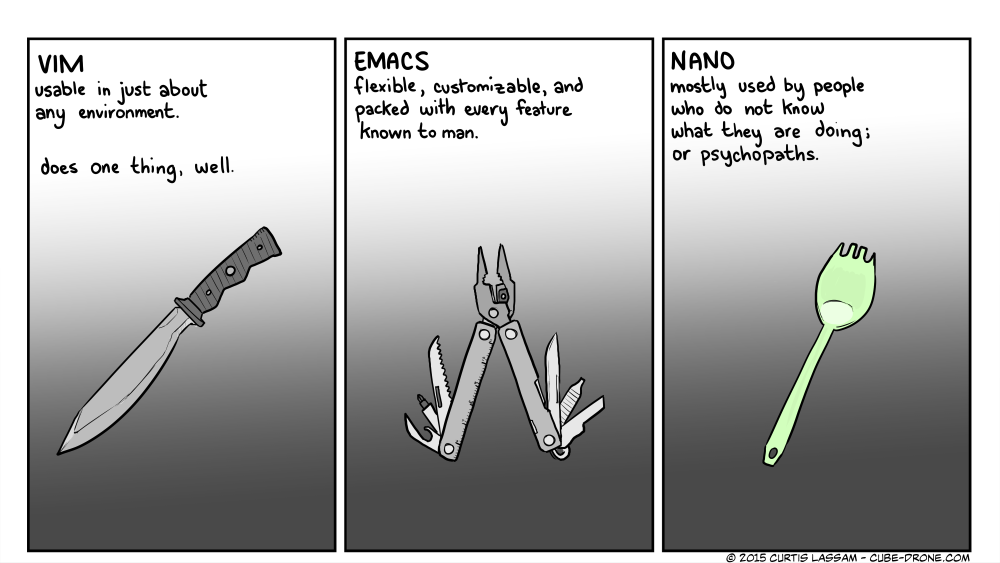
\includegraphics[scale=0.3]{../resources/txt.png}
\end{frame}

\begin{frame}[fragile]
\frametitle{Other tools}

\begin{itemize}
  \item \href{http://www.doxygen.nl/}{\texttt{doxygen}}
  \item \href{https://clang.llvm.org/docs/ClangFormat.html}
    {\texttt{clang-format}}
\end{itemize}

\begin{lstlisting}{bash}
  > sudo apt-get install doxygen clang-format
\end{lstlisting}

If you have installation or setup trouble, consult the \href{https://github.com/umcpt/mc-hammer-2/blob/develop/CONTRIBUTING.md}{contributing} page and the \href{https://github.com/umcpt/mc-hammer-2/tree/develop/docs}{docs}, for setup on specific IDEs, or post in the #help channel on slack.

Most of these tools, as well as several IDEs, are on CAEN windows and RHEL remote desktops, so you can always use those. 


\end{frame}

\section{Contributing a Feature: Lethargy Example}

\subsection{Implementation}

\begin{frame}[fragile]
\frametitle{Clone the repository}

\scriptsize{
\begin{lstlisting}{bash}
>  cd 
>  mkdir demo
>  cd demo
>  git clone git@github.com:umcpt/mc-hammer-2.git

Cloning into 'mc-hammer-2'...
remote: Enumerating objects: 32, done.
remote: Counting objects: 100% (32/32), done.
remote: Compressing objects: 100% (32/32), done.
remote: Total 73802 (delta 5), reused 7 (delta 0), pack-reused 73770
Receiving objects: 100% (73802/73802), 921.70 MiB | 11.72 MiB/s, done.
Resolving deltas: 100% (59832/59832), done.

> cd mc-hammer-2
> ls

CMakeLists.txt   data  examples  README.md  src
CONTRIBUTING.md  docs  extern    scripts    test

> ls src

CMakeLists.txt  geometry  monte_carlo  simulation  sn_solver  utility
\end{lstlisting}}

\end{frame}

\begin{frame}[fragile]
\frametitle{Build the code}

\scriptsize{
\begin{lstlisting}{bash}
> mkdir build
> cd build
> cmake ..
> make -j4 
> make doc
\end{lstlisting}
}
\end{frame}

\begin{frame}[fragile]
\frametitle{Create a feature branch}
A branch is a version of the code. 
They are 'checked out' from an existing branch, changed, 
and then can be `merged` back in. 
The branch types we use are 
\begin{itemize}
  \item feature-<>
  \item test-<>
  \item bugfix-<>
  \item refactor-<>
\end{itemize}

New features are documented in 
\href{https://github.com/umcpt/mc-hammer-2/issues}{Github issues}.

\scriptsize{
\begin{lstlisting}{bash}
> git checkout -b feature-lethargy-calculator
\end{lstlisting}
}
\end{frame}


\begin{frame}[fragile]
\frametitle{Implement the feature}
In \verb|src/utility/lethargy.hpp|:
\scriptsize{
\lstset{language=C++,
                basicstyle=\ttfamily,
                keywordstyle=\color{blue}\ttfamily,
                stringstyle=\color{red}\ttfamily,
                commentstyle=\color{green}\ttfamily,
                morecomment=[l][\color{magenta}]{\#}
}
\begin{lstlisting}{cpp}{
   namespace util {
   /// @brief  Used to calculate the lethargy of an energy
   ///         against a reference energy
   class LethargyCalculator {
   private:
     const double ref_energy;
     
   public:
     LethargyCalculator(double ref_energy) 
     : ref_energy(ref_energy) {}
    
     ///@brief  Calculates lethargy given energy, wrt to ref_energy
     double lethargy(double energy);
   };
   } // namespace util
\end{lstlisting}
}
\end{frame}

\begin{frame}[fragile]
\frametitle{Implement the feature}
In \verb|src/utility/lethargy.cpp|:

\scriptsize{
\lstset{language=C++,
                basicstyle=\ttfamily,
                keywordstyle=\color{blue}\ttfamily,
                stringstyle=\color{red}\ttfamily,
                commentstyle=\color{green}\ttfamily,
                morecomment=[l][\color{magenta}]{\#}
}
\begin{lstlisting}{cpp}
 #include "utility/lethargy.hpp"

 #include <cmath>

 double util::LethargyCalculator::lethargy(double energy) {
   return log(ref_energy / energy);
 }

\end{lstlisting}
}
\end{frame}



\begin{frame}[fragile]
\frametitle{Commit changes}
\tiny{
\begin{lstlisting}{bash}
> git status

On branch feature-lethargy-calculator
Untracked files:
  (use "git add <file>..." to include in what will be committed)

	src/utility/lethargy.cpp
	src/utility/lethargy.hpp

> git add src/utility/lethargy.*
> git status 

On branch feature-lethargy-calculator
Changes to be committed:
  (use "git reset HEAD <file>..." to unstage)
	new file:   src/utility/lethargy.cpp
	new file:   src/utility/lethargy.hpp

> git commit -m "Added the LethargyCalculator class"

[feature-lethargy-calculator 31174ddf1] added the LethargyCalculator class
 2 files changed, 20 insertions(+)
 create mode 100644 src/utility/lethargy.cpp
 create mode 100644 src/utility/lethargy.hpp

> git status 

On branch feature-lethargy-calculator
nothing to commit, working tree clean

\end{lstlisting}
}
\end{frame}

\subsection{Testing}

\begin{frame}[fragile]
\frametitle{Create a test branch}
\scriptsize{
\begin{lstlisting}{bash}
> git checkout -b test-lethargy-calculator
\end{lstlisting}
}
\end{frame}

\begin{frame}[fragile]
\frametitle{Implement the tests}

In \verb|test/utility/test_lethargy.cpp|:

\scriptsize{
\lstset{language=C++,
                basicstyle=\ttfamily,
                keywordstyle=\color{blue}\ttfamily,
                stringstyle=\color{red}\ttfamily,
                commentstyle=\color{green}\ttfamily,
                morecomment=[l][\color{magenta}]{\#}
}
\begin{lstlisting}{cpp}
  #include <catch2/catch.hpp>
   
  #include "utility/lethargy.hpp"
  
  TEST_CASE("LethargyCalculator", "[lethargy]") {
  
    auto myLethargyCalculator = util::LethargyCalculator(1E6);
    REQUIRE( myLethargyCalculator.lethargy(1.0) == Approx(13.81551) );
  }
\end{lstlisting}
}
\end{frame}

\begin{frame}[fragile]
\frametitle{Merge tests into feature branch}
\tiny{
\begin{lstlisting}{bash}
> git add test/utility/test_lethargy.cpp
> git commit -m "added simple test for LethargyCalculator"

[test-lethargy-calculator 0027fa4fd] added simple test for LethargyCalculator
 1 file changed, 9 insertions(+)
 create mode 100644 test/utility/test_lethargy.cpp

> git checkout feature-lethargy-calculator

Switched to branch 'feature-lethargy-calculator'

> git merge test-lethargy-calculator

Updating 31174ddf1..0027fa4fd
Fast-forward
 test/utility/test_lethargy.cpp | 9 +++++++++
 1 file changed, 9 insertions(+)
 create mode 100644 test/utility/test_lethargy.cpp

\end{lstlisting}
}
\end{frame}

\subsection{Merging into develop}

\begin{frame}
\frametitle{Branching}
\centering
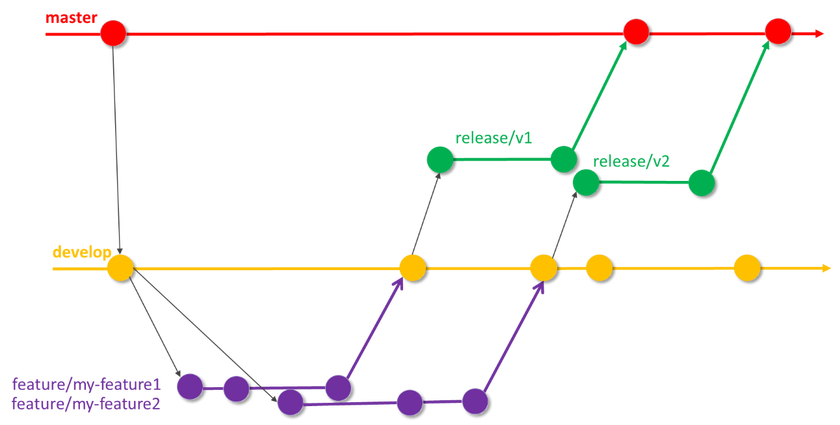
\includegraphics{../resources/branching.png}

\end{frame}

\begin{frame}
\frametitle{Branching}
\centering
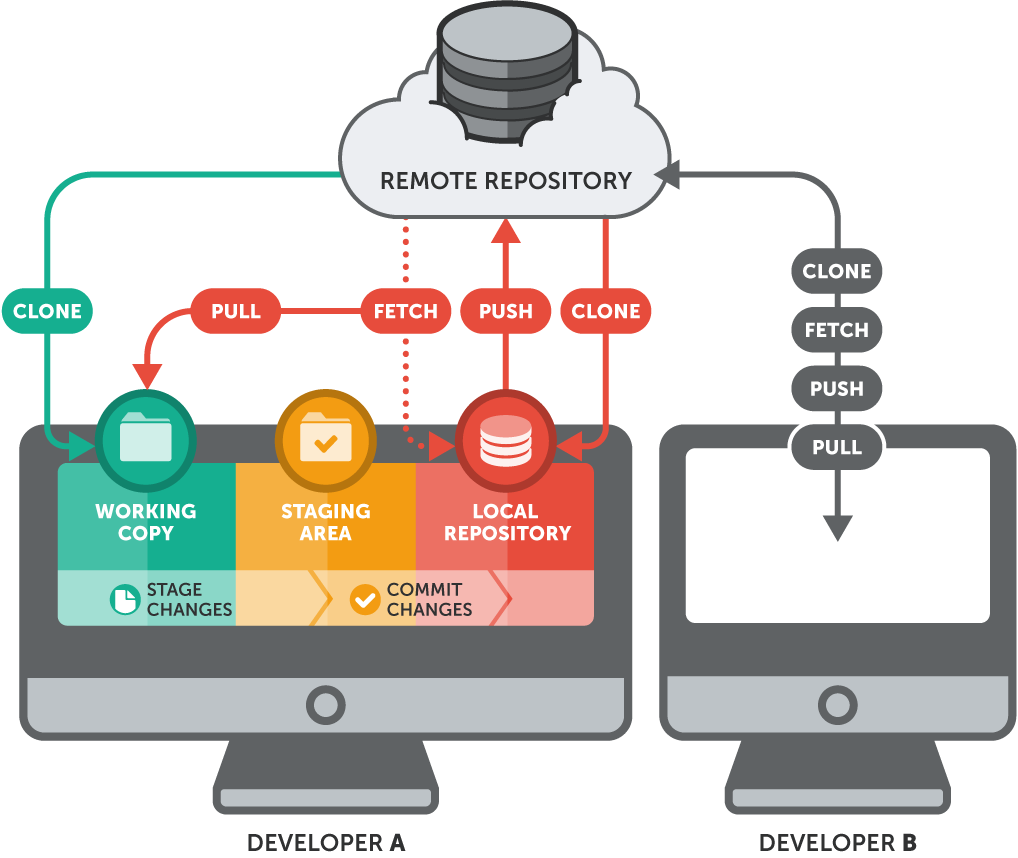
\includegraphics[scale=0.24]{../resources/rem_local.png}

\end{frame}

\begin{frame}[fragile]
\frametitle{Push to remote branch}


This is where the demo stops being interactive!

\vspace{0.5cm}

\normalsize{Now we can push our code, creating a new remote, or upstream, 
branch with the same name.}

\scriptsize{
\begin{lstlisting}{bash}
> git push --set-upstream origin feature-lethargy-calculator
\end{lstlisting}
}

\end{frame}

\begin{frame}
\frametitle{Create a pull request}

\href{https://github.com/umcpt/mc-hammer-2/pulls}{Pull requests} are how we merge code into the develop branch.

PRs should summarize:
\begin{itemize}
  \item what Github issue the PR closes
  \item the feature/bugfix that was implemented
  \item the unit testing that was done
  \item any other changes made to the code
\end{itemize}

While you're working on your feature, you can create a draft pull-request. When you feel it is ready, mark it ``ready for review''.

Make sure you pull from develop early and often!

\end{frame}

\begin{frame}
\frametitle{Code review}

Code reviews are an important tool to maintain code quality. 

\vspace{0.4cm}

Once you submit a PR, you will likely be asked to make changes,
perhaps even several rounds of changes, before you are done with it.

\vspace{0.4cm}

Reviewers should be thorough; checking for code quality, correctness, 
and readability. 
Feature developers should respond to comments promptly.

\end{frame}

\begin{frame}[t]
\frametitle{Helpful Links}
\begin{itemize}
  \item
    \href{https://docs.github.com/en/github/authenticating-to-github/connecting-to-github-with-ssh/generating-a-new-ssh-key-and-adding-it-to-the-ssh-agent}{setting up an SSH key-pair on github to clone the repo}
  \item
  \href{https://github.com/umcpt/mc-hammer-2/blob/develop/CONTRIBUTING.md}{contributing page}
  \item
    \href{https://github.com/umcpt/mc-hammer-2/tree/develop/docs/xcode.md}{xcode setup}
  \item
    \href{https://github.com/umcpt/mc-hammer-2/tree/develop/docs/visual-studio.md}{visual studio setup}
\end{itemize}
  
\end{frame}

\begin{frame}[t]
\frametitle{Current projects}
\begin{itemize}
  \item
    Constructive solid geometry: cell complements, lattices, etc.
  \item
    Photon physics: Incoherent/coherent scatter, photo-electric effect, thick-target Bremstrahlung, pair-production
  \item 
    Neutron physics: (n,$\gamma$), fission, inelastic scatter ENDF laws, thermal scatter on materials, unresolved resonance treatment
  \item
    Machine learning to optimize variance reduction 
\end{itemize}
  
\end{frame}


\end{document} 
